% -*- root: ../VariableReal.tex -*-
\section{¿Por qué necesitamos la integral de Lebesgue?}
\label{sec:MotivacionLebesgue}

Una de las preguntas que nos podemos hacer al estudiar la integral de Lebesgue es por qué es necesaria. Sí, ya sabemos que nos permite integrar cosas como la función de Dirichlet \eqref{eq:Dirichlet}, que recordemos que está dada por la ecuación \[ \mathbb{D}(x) = \begin{cases} 1 & x ∈ ℚ \\ 0 & x ∈ ℝ \setminus ℚ \end{cases} \]

Ahora bien, ¿en qué situaciones nos vamos a encontrar este tipo de ecuaciones? ¿Cuándo nos vamos a topar con una función que tenga deltas de Dirac por ahí? Lo cierto es que no son funciones tan raras como podríamos pensar. De hecho, una curiosidad es que la función de Dirichlet es el límite de funciones continuas: \[ \lim_{n\to ∞} \lim_{m\to ∞} \left[\cos (2πxm!)\right]^n = \mathbb{D}(x) \]

La demostración es ingeniosa: supongamos $x ∈ ℚ$. Entonces, se puede expresar como fracción irreducible $x = \frac{p}{q}$ para algunos $p,q ∈ ℤ$. Al tomar límite, tendremos que a partir de un cierto momento será $m > q$, y por lo tanto $xm! ∈ ℤ$ será entero. Como está multiplicado por $2π$, cuando $x$ sea racional tendremos que ese límite del coseno será $1$ para $x$ racionales (recordemos que $k ∈ ℤ\implies \cos 2πk = 1$).

Para cualquier otro valor de $x$ ($x ∈ ℝ\setminus ℚ$), tendremos que $\cos (2πxm!) < 1$, y al elevarlo a $n$ con $n \to ∞$, el límite en este caso será 0.

En otras palabras, hemos construido una función no sólo discontinua sino además no integrable Riemann sólo con un límite de funciones $C^∞$. Es una muestra de que la integral de Lebesgue nos servirá más allá que para integrar funciones monstruosas inventadas por algún matemático loco.

\section{Funciones continuas no absolutamente continuas}

\begin{figure}[hbtp]
\centering
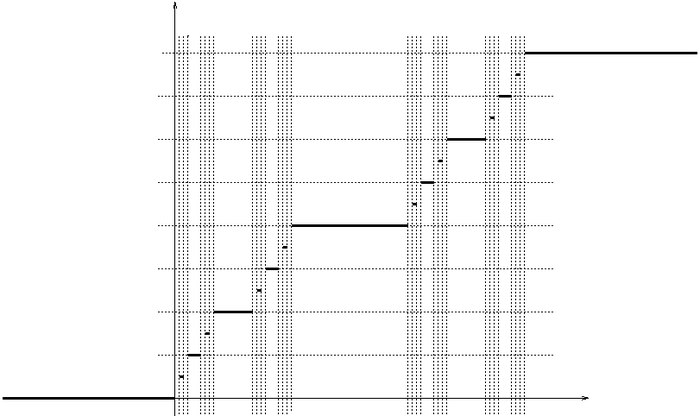
\includegraphics[width=0.8\textwidth]{img/CantorVitaliFunction.png}
\caption{La función de Cantor-Vitali o escalera del diablo.}
\label{fig:CantorVitalFunc}
\end{figure}

Una curiosidad matemática. En la definición de \nlref{def:FuncAbsCont} veíamos que esa era la clase más grande de funciones para las que el teorema fundamental del cálculo con derivada clásica e integral de Lebesgue se cumple. ¿Existe alguna función que sea continua pero no absolutamente continua y que nos sirva de contraejemplo? La respuesta es que sí: es la llamada función de Cantor-Vitali o escalera del diablo.

\begin{defn}[Escalera\IS del diablo] Se construye el conjunto de Cantor y una función que va incrementando en cada ``tercio'' de ese conjunto.
\end{defn}

Sobre el conjunto de Cantor, $f$ es constante, luego $f' = 0$. Sin embargo, la medida del conjunto de Cantor es 1 y por lo tanto la integral no es cero.
